\documentclass{beamer} 


%======================================================================
% Packages / Options
%======================================================================

\usepackage[utf8]{inputenc}

\usepackage[T1]{fontenc}
\usepackage{listings}
\lstset{language=caml,basicstyle=\ttfamily}

% Beamer-specific settings
\mode<presentation>
{
  \usetheme{Darmstadt}
  \useoutertheme{infolines}
}

\AtBeginSection[]
{
  \begin{frame}<beamer>
    \frametitle{Plan}
    \tableofcontents[sectionstyle=show/shaded,subsectionstyle=hide]
  \end{frame}
}

\AtBeginSubsection[]
{
  \begin{frame}<beamer>
    \frametitle{Plan}
    \tableofcontents[sectionstyle=show/hide,subsectionstyle=show/shaded/hide]
  \end{frame}
}

\setbeamertemplate{footline}
{%
\insertpagenumber
\insertshorttitle[width={3cm},center]
\insertshortinstitute[width={3cm},center]
\insertshortdate[width={3cm},center]
}


%======================================================================
% Titlepage
%======================================================================

\title[Analyse Syntaxique]{Analyse Syntaxique}

\author{Mohammed Akram RHAFRANE - Mehdi BOUTCHICHE - Nathanael BERTRAND - Ismail SENHAJI}
\institute{Université de Toulouse III/IRIT}
\date{Année 2012/2013} 

\begin{document}

\begin{frame}
  \titlepage
\end{frame}


%======================================================================
\section{Objectifs du TER}\label{sec:Objectifs}

Initiation à la recherche bibliographique.

Rédaction :
\idem Rapport sur le sujet (40 pages).
\idem Rapport de stage (10 pages).
\idem Présentation du TER.



\frame

% Section 1---------------------------------------------------
\section{Fondamentaux}

\subsection{Langage et grammaire}



\subsection{Analyse Lexicale}



\subsection{Analyse Syntaxique}



\subsubsection{Analyse LL}



\subsubsection{Analyse LR}



% Section 2---------------------------------------------------
\section{Comparaison entre les outils}

\subsection{YACC}



\subsubsection{Définition}



\subsubsection{Exemple}



\subsection{ANTLR}



\subsubsection{Définition}

	\begin{frame}
	\frametitle{Antlr}
 \begin{itemize}
			\item - Générateur de parseur public
			\item - LL(k)
			\item - Framework
			
\end{itemize}
\end{frame} 

\subsubsection{Fonctionnalités}

		\begin{frame}
	\frametitle{Fonctionnalités}
 \begin{itemize}
			\item intègre la spécification entre une analyse lexicale et syntaxique.
			\item facilite la construction de l’arbre syntaxique.
			\item génère des parseurs de descente récursives en C et C++.
			\item facilite la gestion d’erreurs.
			\item ...		
\end{itemize}
\end{frame} 

\subsubsection{Elements du langage}
\begin{frame}
	\frametitle{Elements du langage:}
	
\begin{figure}[h]
	\centering
		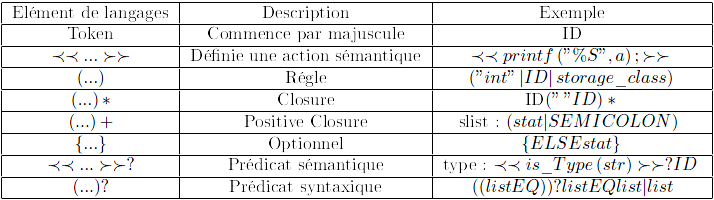
\includegraphics[width=0.80\textwidth]{tabantlr.png}
	\label{fig:tabantlr}
\end{figure}
\end{frame} 


\subsubsection{Exemple}



% Section 3---------------------------------------------------
\section{Xtext}

\subsection{Définition}
	
	 
	
	 
	\begin{frame}
	\frametitle{Xtext}
 \begin{itemize}
			\item - Framework Eclipse
			\item - Développement de langages de programmation et de DSL
			\item - Grammaire proche de celle de Antlr
			\item - Parser LL(*) 
\end{itemize}
\end{frame} 



\subsection{Fonctionnement}

	\begin{frame}
	\frametitle{Diagramme de fonctionnement}
	\begin{figure}[h]
	\centering
		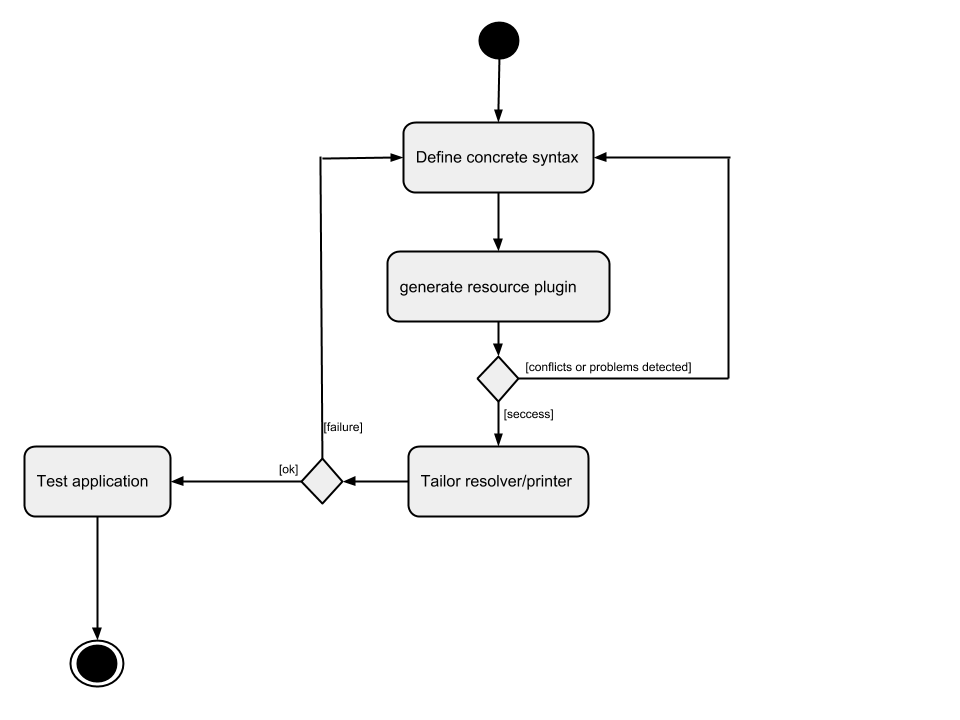
\includegraphics[width=0.80\textwidth]{DiagrammeXtext.png}
	\label{fig:DiagrammeFluxXtext}
\end{figure}

\end{frame} 

\subsection{Exemple}

	\begin{frame}
	\frametitle{Etape 1: Création d'un projet Xtext}
	\begin{figure}[h]
	\centering
			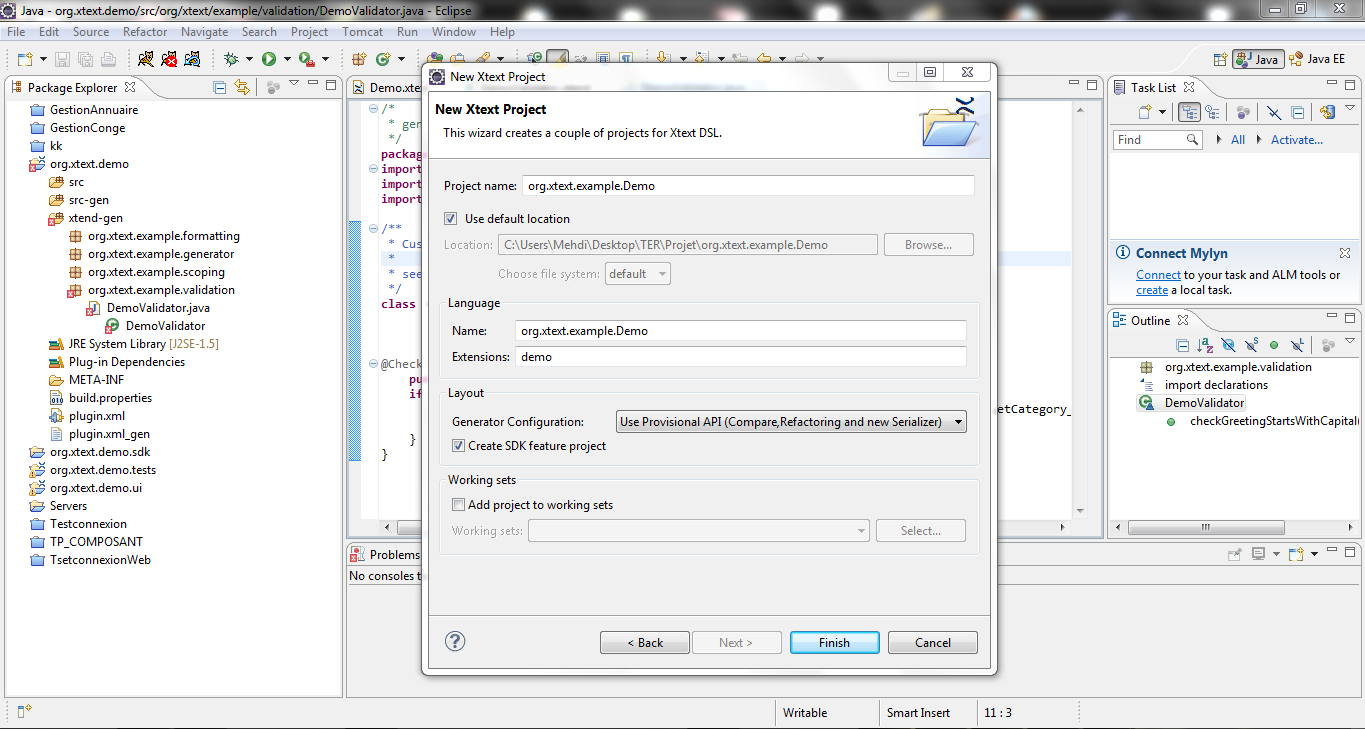
\includegraphics[width=0.90\textwidth]{1.PNG}
	\label{fig:1}
\end{figure}

\end{frame} 


	\begin{frame}
	\frametitle{Etape 2: Definition du langage}
	\begin{figure}[h]
	\centering
			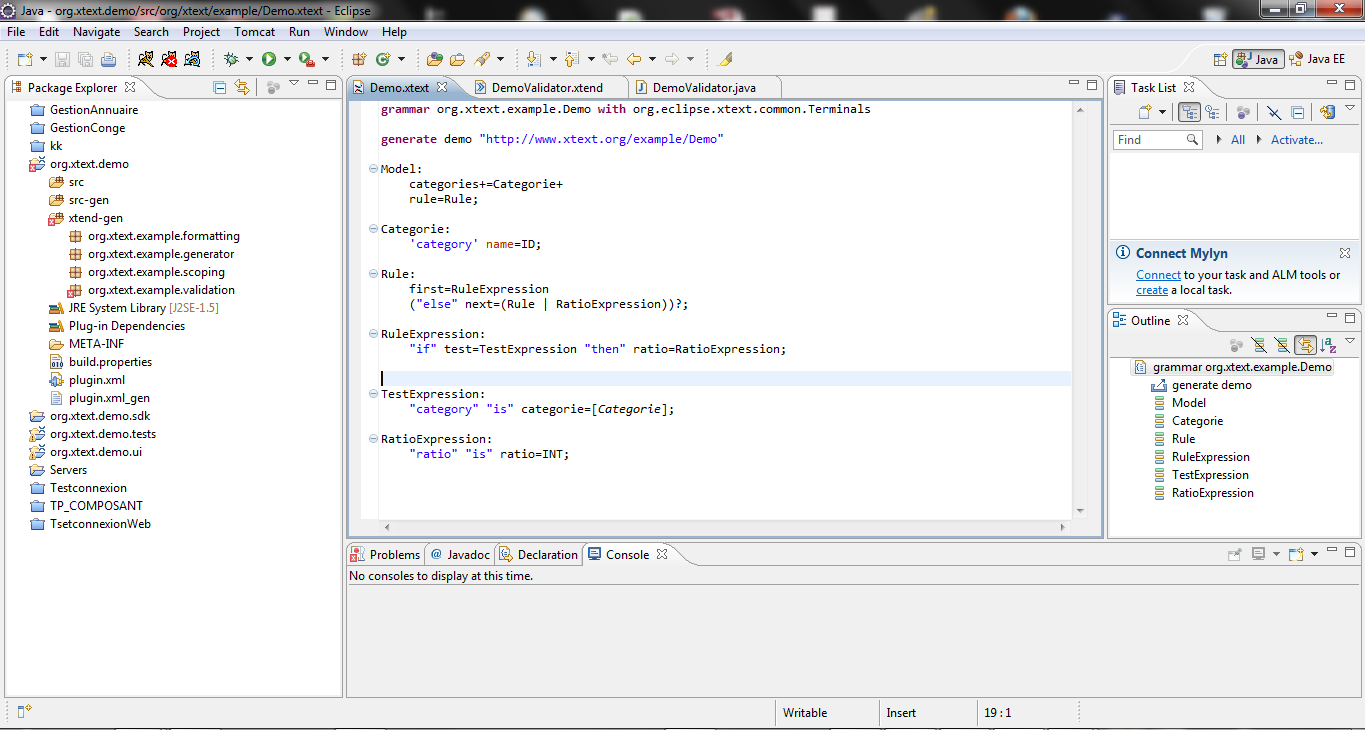
\includegraphics[width=0.90\textwidth]{2.PNG}
	\label{fig:2}
\end{figure}

\end{frame} 

	\begin{frame}
	\frametitle{Etape 3: Generation des artifacts}
	\begin{figure}[h]
	\centering
			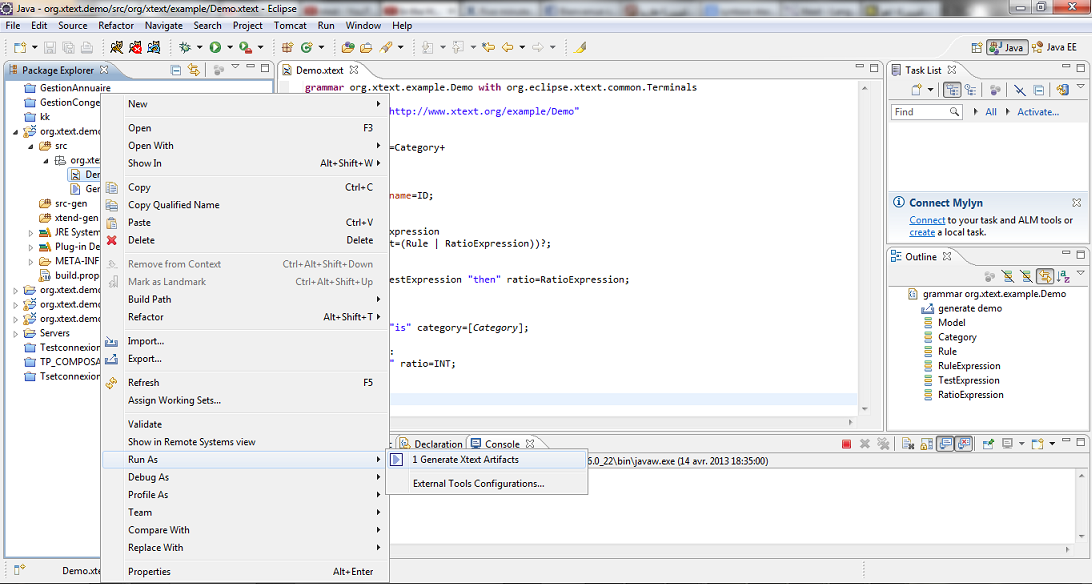
\includegraphics[width=0.90\textwidth]{3.PNG}
	\label{fig:3}
\end{figure}

\end{frame} 
	\begin{frame}
	\frametitle{Etape 4: Faire un test}
	\begin{figure}[h]
	\centering
			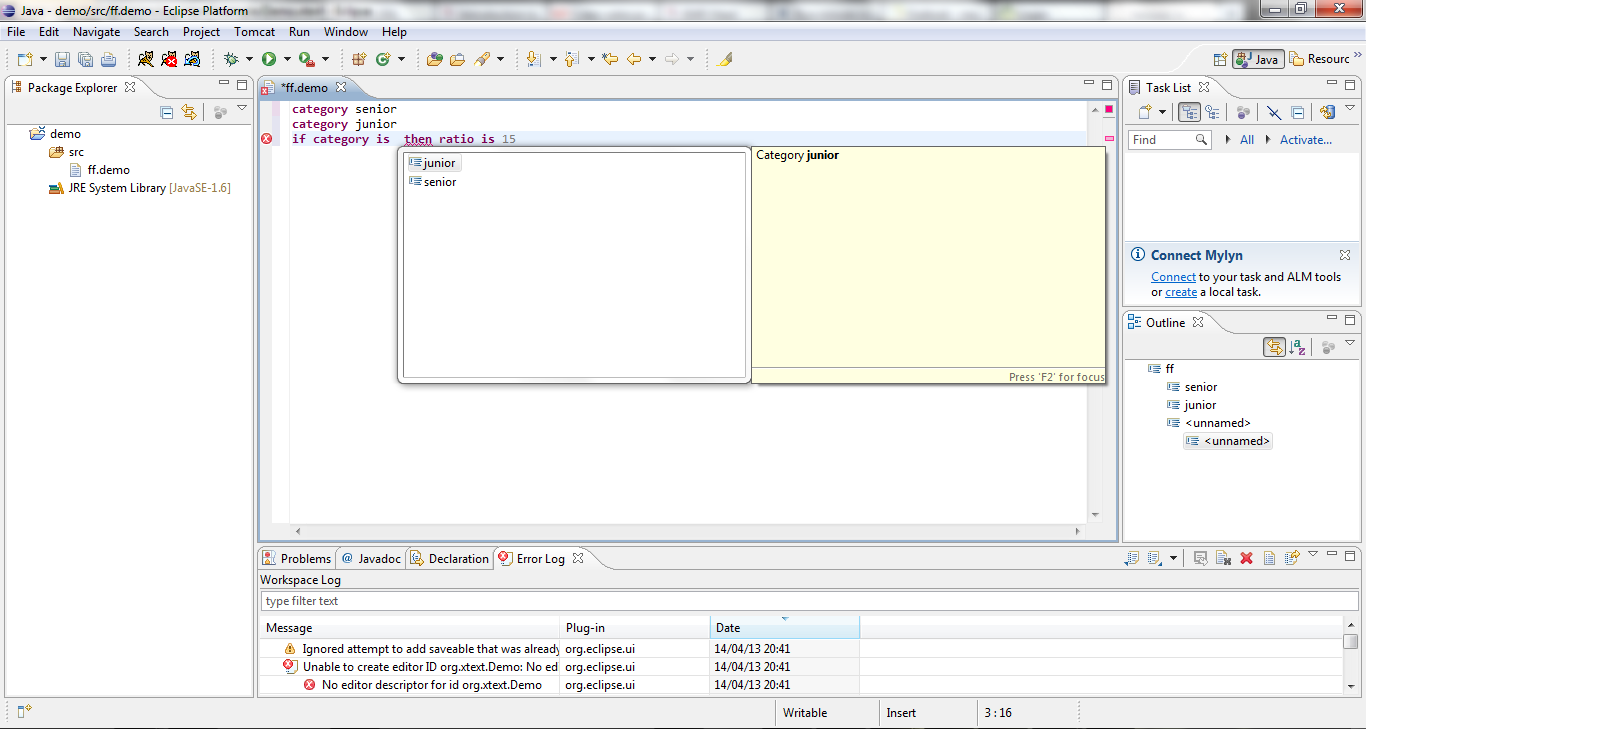
\includegraphics[width=0.90\textwidth]{4.PNG}
	\label{fig:4}
\end{figure}

\end{frame} 	\begin{frame}
	\frametitle{Etape 5: Ajouter une validation}
	\begin{figure}[h]
	\centering
			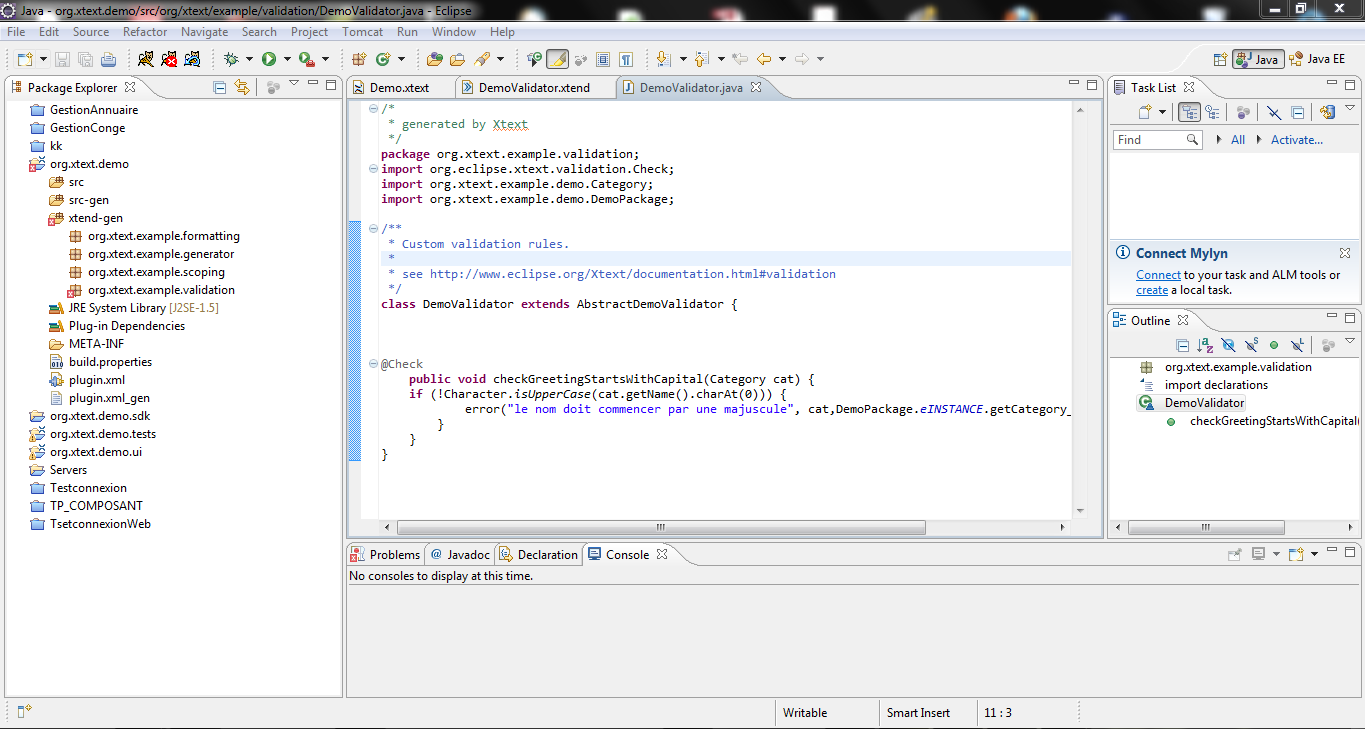
\includegraphics[width=0.90\textwidth]{5.PNG}
	\label{fig:5}
\end{figure}

\end{frame} 

%-------------------------------------------------------------

\section{Conclusion}

\end{document}

%%% Local Variables: 
%%% mode: latex
%%% TeX-master: t
%%% coding: utf-8
%%% End: 
